\documentclass[mathserif, handout]{beamer}

\usepackage{url}
\usepackage{array}
\input{includes}
\input{tikz_figures}

\newcommand{\ttab}[1]{\texttt{#1}}

% draw a row of bit cells: \bitrow{b3/b2/b1/b0}{w3/w2/w1/w0}
% each cell shows a bit, with a weight printed below
\newcommand{\bitcell}[3]{%
  % #1 x-center, #2 bit, #3 weight
  \node[draw, thick, minimum size=8mm, inner sep=0pt] at (#1,0) {\ttab{#2}};
  \node[smallgraytext] at (#1,-0.75) {$#3$};
}

% ------------------------------------------------------------
% multiplication figures
% ------------------------------------------------------------
\usetikzlibrary{arrows.meta, calc, decorations.pathreplacing, shapes.gates.logic.US}

% Column c (c = 0 is the least significant bit) is centred at x = -c*\mpitch,
% so every row lines up on its right edge, as in long multiplication.
\newcommand{\mpitch}{0.72}
\newcommand{\mx}[1]{-(#1)*\mpitch}
\definecolor{bithl}{RGB}{245,194,66}   % swap for the deck's highlight colour

\tikzset{
  mbit/.style     = {draw, thick, minimum size=6mm, inner sep=0pt, font=\ttfamily},
  mbitzero/.style = {mbit, draw=gray!45, text=gray!65},       % a row of zeros
  mbitext/.style  = {mbit, dashed, text=gray!70!black},        % sign extension
  mbitneg/.style  = {mbit, draw=myred, text=myred},            % the subtracted row
  mbitres/.style  = {mbit, very thick, fill=bithl},            % the answer
  mbitdrop/.style = {mbit, dashed, draw=gray!60, text=gray!60},% a dropped carry
  mnote/.style    = {smallgraytext, anchor=west},
  mcarry/.style   = {font=\scriptsize\ttfamily, text=gray},
}

% \mrow[style]{y}{c}{bits}: cells written most significant bit first, with the
% rightmost cell in column c.
\newcommand{\mrow}[4][mbit]{%
  \foreach \mb [count=\n] in {#4} {\xdef\mrowlen{\n}}%
  \foreach \mb [count=\i] in {#4} {%
    \node[#1] at ({\mx{#3 + \mrowlen - \i}}, #2) {\mb};%
  }%
}

% \mrule{y}{c1}{c2}: the line under a sum, from column c1 to column c2,
% extended left to cover the operator.
\newcommand{\mrule}[3]{%
  \draw[thick] ({\mx{#3 + 1} - 0.3}, #1) -- ({\mx{#2} + 0.35}, #1);%
}

% bus-width marks, drawn like the ones in Arithmetic Circuits:
% \mhbus{x}{y}{width} on a horizontal wire, \mvbus{x}{y}{width} on a vertical one
\newcommand{\mhbus}[3]{%
  \draw[thick] ($(#1,#2)+(-0.08,-0.15)$) -- ($(#1,#2)+(0.08,0.15)$);%
  \node[smallgraytext] at ($(#1,#2)+(0,0.32)$) {\ttab{#3}};}
\newcommand{\mvbus}[3]{%
  \draw[thick] ($(#1,#2)+(-0.15,-0.08)$) -- ($(#1,#2)+(0.15,0.08)$);%
  \node[smallgraytext, anchor=west] at ($(#1,#2)+(0.15,0)$) {\ttab{#3}};}

% \mcarry{y}{c}{value}: a carry written above column c
\newcommand{\mcarry}[3]{\node[mcarry] at ({\mx{#2}}, #1) {#3};}

% title
\title{Binary Arithmetic}
\subtitle{Computer Organization}
\author[C. Gummaluru]{Chandra Gummaluru}
\titlegraphic{\includegraphics[width=0.15\linewidth]{images/signature.pdf}}
\institute[]{\url{chandra-gummaluru.github.io} }
\date[Computer Organization]{}

\begin{document}

\begin{frame}
  \maketitle
\end{frame}

\begin{frame}
  \begin{center}
    \highlight{\textbf{number representation}} \\[2mm]
    \graytext{a rule for encoding numbers \\ as patterns of bits}
  \end{center}
\end{frame}

% ------------------------------------------------------------
% unsigned binary
% ------------------------------------------------------------
\begin{frame}{Unsigned Binary}
  \begin{center}
    \Large \highlight{\textbf{unsigned binary}}
  \end{center}
\end{frame}

\begin{frame}
  Each bit stands for a power of two. The value of a pattern is the sum of the weights whose bit is \ttab{1}.\\[6mm]
  \begin{figure}
    \centering
    \begin{tikzpicture}
      \bitcell{0}{1}{8}
      \bitcell{1}{0}{4}
      \bitcell{2}{1}{2}
      \bitcell{3}{1}{1}
    \end{tikzpicture}
  \end{figure}
  \vspace{2mm}
  \begin{center}
    $8 + 2 + 1 = 11$
  \end{center}
With \highlight{n} bits we can represent every whole number from \highlight{0} to \highlight{2^n - 1}.
\end{frame}


\begin{frame}
  To go the other way, we repeatedly divide by two. Each remainder is one bit, read from the last up to the first.\\[3mm]
  \begin{center}
    \renewcommand{\arraystretch}{1.3}
    \begin{tabular}{c@{\hspace{6mm}}c@{\hspace{6mm}}c}
      \graytext{number} & \graytext{halved} & \graytext{remainder} \\ \hline
      \ttab{11} & \ttab{5} & \ttab{1} \\
      \ttab{5}  & \ttab{2} & \ttab{1} \\
      \ttab{2}  & \ttab{1} & \ttab{0} \\
      \ttab{1}  & \ttab{0} & \ttab{1} \\
    \end{tabular}
  \end{center}
  \vspace{2mm}
  \begin{center}
    \graytext{reading the remainders upward gives}\hspace{2mm}\highlight{\ttab{1011}}
  \end{center}
\end{frame}

% ------------------------------------------------------------
% hexadecimal
% ------------------------------------------------------------
\begin{frame}{Hexadecimal}
  \begin{center}
    \Large \highlight{\textbf{hexadecimal}}
  \end{center}
\end{frame}

\begin{frame}
  Long bit patterns are hard to read. \highlight{\textbf{Hexadecimal}} replaces each group of four bits with one symbol.\\[4mm]
  \begin{center}
    \renewcommand{\arraystretch}{1.2}
    \begin{tabular}{cc@{\hspace{10mm}}cc}
      \graytext{bits} & \graytext{hex} & \graytext{bits} & \graytext{hex} \\ \hline
      \ttab{0000} & \ttab{0} & \ttab{1000} & \ttab{8} \\
      \ttab{0001} & \ttab{1} & \ttab{1001} & \ttab{9} \\
      \ttab{0010} & \ttab{2} & \ttab{1010} & \ttab{A} \\
      \ttab{0011} & \ttab{3} & \ttab{1011} & \ttab{B} \\
      \ttab{0100} & \ttab{4} & \ttab{1100} & \ttab{C} \\
      \ttab{0101} & \ttab{5} & \ttab{1101} & \ttab{D} \\
      \ttab{0110} & \ttab{6} & \ttab{1110} & \ttab{E} \\
      \ttab{0111} & \ttab{7} & \ttab{1111} & \ttab{F} \\
    \end{tabular}
  \end{center}
\end{frame}

\begin{frame}
  We split the bits into groups of four and write the symbol for each group.\\[6mm]
  \begin{center}
    \ttab{1011} \; \ttab{0110} \\[2mm]
    \graytext{becomes} \\[2mm]
    \highlight{\ttab{B6}}
  \end{center}
\end{frame}

% ------------------------------------------------------------
% two's complement
% ------------------------------------------------------------
\begin{frame}{Signed Numbers}
  \begin{center}
    \Large \highlight{\textbf{signed numbers}}
  \end{center}
\end{frame}

\begin{frame}{Representing Negative Numbers}

  With fixed-length numbers, a negative
  value has to be represented by a \emph{positive} bit pattern.
  \\~\\
  Given a number $n$, we define its negation $-n$ as any number satisfying
    \[
      n + (-n) = 0 .
    \]
\end{frame}

\begin{frame}
  To negate a decimal number, we take two steps.\\[5mm]
  \begin{center}
    \renewcommand{\arraystretch}{1.5}
    \begin{tabular}{r@{\hspace{6mm}}l}
      \ttab{49}          & \graytext{the value \ttab{49}} \\
      \ttab{50}          & \graytext{subtract each digit from \ttab{9}} \\
      \ttab{51}          & \graytext{add one, giving a representation of \ttab{-49}} \\
    \end{tabular}
  \end{center}
\end{frame}

% Fixed-width numbers wrap around: the circle behind "invert and add one".
% Value v sits at angle 90 - 36v, so 0 is at the top and counting runs clockwise.
\begin{frame}
  Fixed-width numbers live on a \highlight{\textbf{circle}}: counting past the largest value wraps back to \ttab{0}. With one digit, \ttab{9} is one step before \ttab{0}, so it acts as $-1$.\\[3mm]
  \begin{minipage}{0.5\textwidth}
    \centering
    \begin{tikzpicture}[scale=0.85, >={Stealth[length=2.2mm]}]
      \draw[thick, gray!60] (0,0) circle (1.5);
      \foreach \v in {0,...,9} {
        \fill ({90-36*\v}:1.5) circle (1.6pt);
        \node[font=\ttfamily] at ({90-36*\v}:1.88) {\v};
      }
      % the values that stand for negatives
      \node[smallgraytext] at (126:1.08) {$-1$};
      \node[smallgraytext, text=myred] at (234:1.08) {$-4$};

      % 9 - 4 = 5: back four steps from 9, never passing 0, so no borrows
      \draw[->, thick, gray] (126:2.3) arc[start angle=126, end angle=266, radius=2.3];
      \node[smallgraytext, anchor=east] at (190:2.4) {$9 - 4$};
      % then one step forward
      \draw[->, very thick, myred] (270:2.75) arc[start angle=270, end angle=236, radius=2.75];
      \node[smallgraytext, text=myred, anchor=north] at (258:2.85) {$+1$};

      % the same place, reached directly: 0 - 4 wraps round to 6
      \draw[->, thick, dashed, gray] (90:0.62) arc[start angle=90, end angle=228, radius=0.62];
      \node[smallgraytext] at (0.1,-0.05) {$0 - 4$};
    \end{tikzpicture}
  \end{minipage}%
  \begin{minipage}{0.5\textwidth}
    \ttab{9 - 4 = 5} \\
    \graytext{\small subtract from \ttab{9}: never a borrow} \\[3mm]
    \ttab{5 + 1 = 6} \\
    \graytext{\small add one} \\[5mm]
    \ttab{6} lands where \ttab{0 - 4} does, so \ttab{6} stands for $-4$. \\[1mm]
    \graytext{\small $4 + 6 = 10$, which wraps to \ttab{0}}
  \end{minipage}
  \vspace{4mm}
  \begin{center}
    \graytext{with two digits the circle has 100 steps: $99 - 49 = 50$, then $+1$ gives $51 \equiv -49$}
  \end{center}
\end{frame}

\begin{frame}
  To negate a binary number we take two similar steps.\\[5mm]
  \begin{center}
    \renewcommand{\arraystretch}{1.5}
    \begin{tabular}{r@{\hspace{6mm}}l}
      \ttab{0101}          & \graytext{the value \ttab{5}} \\
      \ttab{1010}          & \graytext{subtract each bit from \texttt{1} (invert each bit)} \\
      \ttab{1011}          & \graytext{add one, giving a representation of \ttab{-5}} \\
    \end{tabular}
  \end{center}
This is called \highlight{\textbf{twos-complement}}.
  \begin{figure}
    \centering
    \begin{tikzpicture}
      \node[draw, thick, minimum size=8mm, inner sep=0pt] at (0,0) {\ttab{1}};
      \node[smallgraytext, text=myred] at (0,-0.75) {$-8$};
      \bitcell{1}{0}{4}
      \bitcell{2}{1}{2}
      \bitcell{3}{1}{1}
    \end{tikzpicture}
  \end{figure}
\end{frame}

\begin{frame}
  Adding one to all-ones rolls over to zero, so all-ones must be \ttab{-1}.\\[4mm]
  \begin{center}
    \renewcommand{\arraystretch}{1.3}
    \begin{tabular}{r@{\hspace{2mm}}l}
       & \ttab{1111} \\
      $+$ & \ttab{0001} \\ \hline
      \ttab{1} & \ttab{0000} \\
    \end{tabular}
  \end{center}
\end{frame}

\begin{frame}
  With \highlight{$n$} bits, two's complement covers a balanced range around zero.\\[4mm]
  \begin{center}
    \highlight{-2^{n-1}} \graytext{ to } \highlight{2^{n-1} - 1}
  \end{center}
  \vspace{3mm}
  \begin{center}
    \graytext{four bits run from \ttab{-8} to \ttab{7}}
  \end{center}
\end{frame}

% ------------------------------------------------------------
% addition
% ------------------------------------------------------------
\begin{frame}{Addition}
  \begin{center}
    \Large \highlight{\textbf{addition}}
  \end{center}
\end{frame}

\begin{frame}
  We add binary numbers one column at a time, from the right, just as in decimal. A column can add up to at most three, so it always gives one bit to write and at most one to carry.\\[5mm]
  \begin{center}
    \renewcommand{\arraystretch}{1.5}
    \begin{tabular}{r@{\hspace{3mm}}c@{\hspace{3mm}}l@{\hspace{10mm}}l}
      \ttab{0 + 0}     & $=$ & \ttab{\phantom{1}0} & \graytext{write \ttab{0}} \\
      \ttab{0 + 1}     & $=$ & \ttab{\phantom{1}1} & \graytext{write \ttab{1}} \\
      \ttab{1 + 1}     & $=$ & \ttab{10}           & \graytext{write \ttab{0}, carry \ttab{1}} \\
      \ttab{1 + 1 + 1} & $=$ & \ttab{11}           & \graytext{write \ttab{1}, carry \ttab{1}} \\
    \end{tabular}
  \end{center}
  \vspace{2mm}
  \begin{center}
    \graytext{the third \ttab{1} is a carry coming in from the column to the right}
  \end{center}
\end{frame}

\begin{frame}
  To add \ttab{0101} (5) and \ttab{0011} (3), we work right to left, writing each column's carry above the next.\\[5mm]
  \begin{center}
    \begin{tikzpicture}
      \mrow[smallgraytext]{0.95}{0}{8,4,2,1}
      \uncover<3->{\mcarry{0.5}{1}{1}}
      \uncover<4->{\mcarry{0.5}{2}{1}}
      \uncover<5->{\mcarry{0.5}{3}{1}}
      \mrow{0}{0}{0,1,0,1}      \node[mnote] at (0.45, 0) {$5$};
      \mrow{-0.75}{0}{0,0,1,1}  \node[mnote] at (0.45, -0.75) {$3$};
      \node at ({\mx{4}}, -0.75) {$+$};
      \mrule{-1.15}{0}{3}
      \foreach \col/\bitv [count=\stp from 2] in {0/0,1/0,2/0,3/1}
        {\uncover<\stp->{\node[mbitres] at ({\mx{\col}}, -1.6) {\bitv};}}
      \uncover<5->{\node[mnote] at (0.45, -1.6) {$= 8$};}
    \end{tikzpicture}
  \end{center}
  \vspace{3mm}
  \begin{center}
    \graytext{each \ttab{1 + 1} writes \ttab{0} and carries \ttab{1} into the next column}
  \end{center}
\end{frame}

\begin{frame}
  With $n$ bits, a sum can need $n + 1$. The extra bit is the \highlight{\textbf{carry out}}; the result keeps only $n$ bits, so the carry out is lost.\\[5mm]
  \begin{center}
    \begin{tikzpicture}
      \mrow[smallgraytext]{0.95}{0}{8,4,2,1}
      \mcarry{0.5}{4}{1}
      \mrow{0}{0}{1,0,0,1}      \node[mnote] at (0.45, 0) {$9$};
      \mrow{-0.75}{0}{1,1,0,0}  \node[mnote] at (0.45, -0.75) {$12$};
      \node at ({\mx{5}}, -0.75) {$+$};
      \mrule{-1.15}{0}{4}
      \node[mbitdrop] at ({\mx{4}}, -1.6) {1};
      \mrow[mbitres]{-1.6}{0}{0,1,0,1}
      \node[mnote] at (0.45, -1.6) {$= 5$, \graytext{not $21$}};
      \node[smallgraytext, anchor=north] at ({\mx{4}}, -1.95) {carry out};
    \end{tikzpicture}
  \end{center}
  \vspace{3mm}
  \begin{center}
    \graytext{for unsigned numbers, a carry out of \ttab{1} means the sum did not fit}
  \end{center}
\end{frame}

\begin{frame}
  Two's-complement numbers add in exactly the same way. The carry out is still dropped, but here the answer is right.\\[5mm]
  \begin{center}
    \begin{tikzpicture}
      \node[smallgraytext, text=myred] at ({\mx{3}}, 0.95) {$-8$};
      \mrow[smallgraytext]{0.95}{0}{4,2,1}
      \mcarry{0.5}{3}{1} \mcarry{0.5}{4}{1}
      \mrow{0}{0}{1,1,0,1}      \node[mnote] at (0.45, 0) {$-3$};
      \mrow{-0.75}{0}{1,1,1,0}  \node[mnote] at (0.45, -0.75) {$-2$};
      \node at ({\mx{5}}, -0.75) {$+$};
      \mrule{-1.15}{0}{4}
      \node[mbitdrop] at ({\mx{4}}, -1.6) {1};
      \mrow[mbitres]{-1.6}{0}{1,0,1,1}
      \node[mnote] at (0.45, -1.6) {$= -5$};
    \end{tikzpicture}
  \end{center}
  \vspace{3mm}
  \begin{center}
    \graytext{the same adder serves both readings; only the check for a wrong answer differs}
  \end{center}
\end{frame}

\begin{frame}
  When two numbers of the same sign give a result of the other sign, the answer has \highlight{\textbf{overflowed}}.\\[5mm]
  \begin{center}
    \begin{tikzpicture}
      \node[smallgraytext, text=myred] at ({\mx{3}}, 0.95) {$-8$};
      \mrow[smallgraytext]{0.95}{0}{4,2,1}
      \node[mcarry, text=myred] at ({\mx{3}}, 0.5) {1};
      \node[mcarry, text=myred] at ({\mx{4}}, 0.5) {0};
      \mrow{0}{0}{0,1,0,1}      \node[mnote] at (0.45, 0) {$5$};
      \mrow{-0.75}{0}{0,1,0,0}  \node[mnote] at (0.45, -0.75) {$4$};
      \node at ({\mx{5}}, -0.75) {$+$};
      \mrule{-1.15}{0}{4}
      \mrow[mbitres]{-1.6}{0}{1,0,0,1}
      \node[mnote] at (0.45, -1.6) {$= -7$, \graytext{not $9$}};
    \end{tikzpicture}
  \end{center}
  \vspace{3mm}
  \begin{center}
    \graytext{the carry into the sign bit (\ttab{1}) differs from the carry out of it (\ttab{0})}
  \end{center}
\end{frame}

% ------------------------------------------------------------
% subtraction
% ------------------------------------------------------------
\begin{frame}{Subtraction}
  \begin{center}
    \Large \highlight{\textbf{subtraction}}
  \end{center}
\end{frame}

\begin{frame}
  We subtract by adding the negation: \highlight{a - b = a + (-b)}. To negate \ttab{b}, we invert every bit, then add one.\\[5mm]
  \begin{center}
    \begin{tikzpicture}
      \mrow{0}{0}{0,0,1,1}          \node[mnote] at (0.45, 0) {$3$};
      \draw[-{Stealth[length=2mm]}, gray] ({\mx{1.5}}, -0.4) -- ({\mx{1.5}}, -0.85)
        node[midway, left=10mm, smallgraytext] {invert every bit};
      \mrow{-1.25}{0}{1,1,0,0}      \node[mnote] at (0.45, -1.25) {$-4$};
      \draw[-{Stealth[length=2mm]}, gray] ({\mx{1.5}}, -1.65) -- ({\mx{1.5}}, -2.1)
        node[midway, left=10mm, smallgraytext] {add one};
      \mrow[mbitres]{-2.5}{0}{1,1,0,1}  \node[mnote] at (0.45, -2.5) {$-3$};
    \end{tikzpicture}
  \end{center}
  \vspace{3mm}
  \begin{center}
    \graytext{then an ordinary addition finishes the job}
  \end{center}
\end{frame}

\begin{frame}
  To compute \ttab{0101} $-$ \ttab{0011} (5 $-$ 3), we add \ttab{0101} and $-3$ = \ttab{1101}.\\[5mm]
  \begin{center}
    \begin{tikzpicture}
      \mrow[smallgraytext]{0.95}{0}{8,4,2,1}
      \uncover<2->{\mcarry{0.5}{1}{1}}
      \uncover<4->{\mcarry{0.5}{3}{1}}
      \uncover<5->{\mcarry{0.5}{4}{1}}
      \mrow{0}{0}{0,1,0,1}      \node[mnote] at (0.45, 0) {$5$};
      \mrow{-0.75}{0}{1,1,0,1}  \node[mnote] at (0.45, -0.75) {$-3$};
      \node at ({\mx{5}}, -0.75) {$+$};
      \mrule{-1.15}{0}{4}
      \foreach \col/\bitv [count=\stp from 2] in {0/0,1/1,2/0,3/0}
        {\uncover<\stp->{\node[mbitres] at ({\mx{\col}}, -1.6) {\bitv};}}
      \uncover<5->{
        \node[mbitdrop] at ({\mx{4}}, -1.6) {1};
        \node[mnote] at (0.45, -1.6) {$= 2$};}
    \end{tikzpicture}
  \end{center}
  \vspace{3mm}
  \begin{center}
    \graytext{the carry out is dropped, as in any addition}
  \end{center}
\end{frame}

\begin{frame}
  For unsigned numbers, the carry out now tells us whether we had to \highlight{\textbf{borrow}}: it is \ttab{1} when $a \ge b$ and \ttab{0} when $a < b$.\\[5mm]
  \begin{center}
    \begin{tikzpicture}[scale=0.88, transform shape]
      % 7 - 5
      \begin{scope}[xshift=-2.6cm]
        \mrow{0}{0}{0,1,1,1}      \node[mnote] at (0.45, 0) {$7$};
        \mrow{-0.75}{0}{1,0,1,1}  \node[mnote] at (0.45, -0.75) {$-5$};
        \node at ({\mx{5}}, -0.75) {$+$};
        \mrule{-1.15}{0}{4}
        \node[mbitext] at ({\mx{4}}, -1.6) {1};
        \mrow[mbitres]{-1.6}{0}{0,0,1,0}
        \node[mnote] at (0.45, -1.6) {$= 2$};
        \node[smallgraytext, anchor=north, align=center] at ({\mx{2}}, -2.05) {carry out \ttab{1}: \\ no borrow, correct};
      \end{scope}
      % 5 - 7
      \begin{scope}[xshift=4.2cm]
        \mrow{0}{0}{0,1,0,1}      \node[mnote] at (0.45, 0) {$5$};
        \mrow{-0.75}{0}{1,0,0,1}  \node[mnote] at (0.45, -0.75) {$-7$};
        \node at ({\mx{5}}, -0.75) {$+$};
        \mrule{-1.15}{0}{4}
        \node[mbitext] at ({\mx{4}}, -1.6) {0};
        \mrow[mbitres]{-1.6}{0}{1,1,1,0}
        \node[mnote] at (0.45, -1.6) {$= 14$};
        \node[smallgraytext, anchor=north, align=center] at ({\mx{2}}, -2.05) {carry out \ttab{0}: \\ a borrow, not $-2$};
      \end{scope}
    \end{tikzpicture}
  \end{center}
\end{frame}

\begin{frame}
  Signed subtraction overflows when \ttab{a} and \ttab{b} have different signs and the result's sign isn't \ttab{a}'s.\\[5mm]
  \begin{center}
    \begin{tikzpicture}
      \node[smallgraytext, text=myred] at ({\mx{3}}, 0.95) {$-8$};
      \mrow[smallgraytext]{0.95}{0}{4,2,1}
      \mcarry{0.5}{3}{1}
      \mrow{0}{0}{0,1,0,1}      \node[mnote] at (0.45, 0) {$5$};
      \mrow{-0.75}{0}{0,1,0,0}  \node[mnote] at (0.45, -0.75) {$-(-4) = 4$};
      \node at ({\mx{5}}, -0.75) {$+$};
      \mrule{-1.15}{0}{4}
      \mrow[mbitres]{-1.6}{0}{1,0,0,1}
      \node[mnote] at (0.45, -1.6) {$= -7$, \graytext{not $9$}};
    \end{tikzpicture}
  \end{center}
  \vspace{3mm}
  \begin{center}
    \graytext{it overflows exactly when the addition $a + (-b)$ does}
  \end{center}
\end{frame}

\begin{frame}
  The same adder does all four, with \ttab{a - b} computed as \mbox{\ttab{a + \textasciitilde b + 1}}. Only our reading of the bits changes, and with it how we tell the answer is \highlight{\textbf{wrong}}.\\[4mm]
  \begin{center}
    \small
    \renewcommand{\arraystretch}{1.4}
    \begin{tabular}{l@{\hspace{4mm}}>{\raggedright\arraybackslash\leavevmode}p{3.6cm}@{\hspace{4mm}}l}
      & \graytext{wrong when} & \graytext{example (4 bits)} \\ \hline
      \textbf{unsigned} \ttab{a + b}
        & \ttab{cout = 1}
        & \ttab{9 + 12} $\to$ \ttab{0101} \graytext{(5)} \\
      \textbf{unsigned} \ttab{a - b}
        & \ttab{cout = 0} \graytext{(a borrow)}
        & \ttab{5 - 7} $\to$ \ttab{1110} \graytext{(14)} \\
      \textbf{signed} \ttab{a + b}
        & \graytext{inputs share a sign, the result has the other}
        & \ttab{5 + 4} $\to$ \ttab{1001} \graytext{(-7)} \\
      \textbf{signed} \ttab{a - b}
        & \graytext{inputs differ in sign, the result's sign isn't \ttab{a}'s}
        & \ttab{5 - (-4)} $\to$ \ttab{1001} \graytext{(-7)} \\
    \end{tabular}
  \end{center}
  \vspace{3mm}
  \begin{center}
    \graytext{unsigned checks \ttab{carry}; signed checks \ttab{overflow} (\ttab{cin} $\neq$ \ttab{cout} at the sign bit)}
  \end{center}
\end{frame}

% ------------------------------------------------------------
% multiplication
% ------------------------------------------------------------
\begin{frame}{Multiplication}
  \begin{center}
    \Large \highlight{\textbf{multiplication}}
  \end{center}
\end{frame}

\begin{frame}
  In decimal long multiplication, we multiply by one digit at a time, shift each row one place further left, and add the rows.\\[5mm]
  \begin{center}
    \renewcommand{\arraystretch}{1.3}
    \begin{tabular}{r@{\hspace{2mm}}r@{\hspace{8mm}}l}
               & \ttab{12} & \\
      $\times$ & \ttab{13} & \\ \cline{1-2}
               & \ttab{36} & \graytext{$12 \times 3$} \\
      $+$      & \ttab{12{\color{gray}0}} & \graytext{$12 \times 1$, shifted one place} \\ \cline{1-2}
               & \ttab{156} & \\
    \end{tabular}
  \end{center}
  \vspace{4mm}
  \begin{center}
    \graytext{binary works the same way, with much simpler rows}
  \end{center}
\end{frame}

\begin{frame}
  Every binary digit is \ttab{0} or \ttab{1}, so each row is either a copy of the first number or all zeros.\\[6mm]
  \begin{center}
    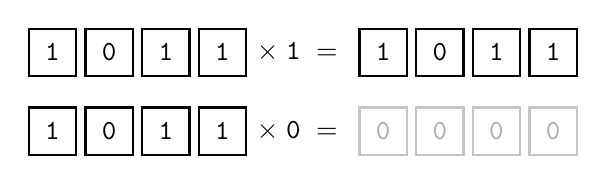
\begin{tikzpicture}
      \mrow{0}{0}{1,0,1,1}
      \node at (0.95, 0) {$\times\;\ttab{1}\;=$};
      \begin{scope}[xshift=4.2cm]
        \mrow{0}{0}{1,0,1,1}
      \end{scope}
      \mrow{-1}{0}{1,0,1,1}
      \node at (0.95, -1) {$\times\;\ttab{0}\;=$};
      \begin{scope}[xshift=4.2cm]
        \mrow[mbitzero]{-1}{0}{0,0,0,0}
      \end{scope}
    \end{tikzpicture}
  \end{center}
  \vspace{4mm}
  Each bit of a row is \ttab{1} only when both bits are \ttab{1}: an \highlight{\textbf{AND}}.
  \begin{center}
    \begin{tikzpicture}
      \node[and gate US, draw, thick, scale=1.3] (g) at (0,0) {};
      \draw[thick] (g.input 1) -- ++(-0.3,0) |- ++(-0.5,0.25) node[left] {$a_i$};
      \draw[thick] (g.input 2) -- ++(-0.3,0) |- ++(-0.5,-0.25) node[left] {$b_j$};
      \draw[thick] (g.output) -- ++(0.6,0) node[right] {$a_i \cdot b_j$};
      \node[smallgraytext, anchor=west, align=left] at (2.7, 0) {one gate per bit \\ builds every row at once};
    \end{tikzpicture}
  \end{center}
\end{frame}

\begin{frame}
  Shifting every bit one place left moves it to a weight twice as large, so the value doubles.\\[6mm]
  \begin{center}
    \begin{tikzpicture}
      \foreach \w [count=\col from 0] in {1,2,4,8,16}
        \node[smallgraytext] at ({\mx{\col}}, 0.6) {$\w$};
      \mrow{0}{0}{0,0,1,1}
      \node[mnote] at (0.45, 0) {$= 3$};
      \mrow{-1.6}{1}{0,1,1}
      \node[mbitres] at ({\mx{0}}, -1.6) {0};
      \node[mbitzero] at ({\mx{4}}, -1.6) {0};
      \node[mnote] at (0.45, -1.6) {$= 6$};
      \foreach \col in {0,1,2,3}
        \draw[-{Stealth[length=2mm]}, gray] ({\mx{\col}}, -0.35) -- ({\mx{\col+1}}, -1.25);
      \node[smallgraytext, anchor=north] at ({\mx{0}}, -1.95) {a \ttab{0} fills in};
    \end{tikzpicture}
  \end{center}
  \vspace{4mm}
  \begin{center}
    \graytext{shifting left by $k$ places multiplies by $2^k$}
  \end{center}
\end{frame}

\begin{frame}
  To multiply \ttab{1011} (11) by \ttab{1101} (13), we write one row for each bit of the second number, shifted left by that bit's position.\\[4mm]
  \begin{center}
    \begin{tikzpicture}
      \mrow{0}{0}{1,0,1,1}
      \mrow{-0.8}{0}{1,1,0,1}
      \node at ({\mx{4}}, -0.8) {$\times$};
      % the bit of the second number that picks the current row
      \only<2| handout:0>{\node[draw=bithl, line width=2pt, minimum size=7.6mm] at ({\mx{0}}, -0.8) {};}
      \only<3| handout:0>{\node[draw=bithl, line width=2pt, minimum size=7.6mm] at ({\mx{1}}, -0.8) {};}
      \only<4| handout:0>{\node[draw=bithl, line width=2pt, minimum size=7.6mm] at ({\mx{2}}, -0.8) {};}
      \only<5| handout:0>{\node[draw=bithl, line width=2pt, minimum size=7.6mm] at ({\mx{3}}, -0.8) {};}
      \mrule{-1.25}{0}{6}

      \uncover<2->{
        \mrow{-1.75}{0}{1,0,1,1}
        \node[mnote] at (0.45, -1.75) {bit 0 is \ttab{1}: copy};}
      \uncover<3->{
        \node at ({\mx{7}}, -2.55) {$+$};
        \mrow[mbitzero]{-2.55}{1}{0,0,0,0}
        \node[mnote] at (0.45, -2.55) {bit 1 is \ttab{0}: zeros};}
      \uncover<4->{
        \node at ({\mx{7}}, -3.35) {$+$};
        \mrow{-3.35}{2}{1,0,1,1}
        \node[mnote] at (0.45, -3.35) {bit 2 is \ttab{1}: copy, shifted 2};}
      \uncover<5->{
        \node at ({\mx{7}}, -4.15) {$+$};
        \mrow{-4.15}{3}{1,0,1,1}
        \node[mnote] at (0.45, -4.15) {bit 3 is \ttab{1}: copy, shifted 3};}
    \end{tikzpicture}
  \end{center}
\end{frame}

\begin{frame}
  Then we add the rows, one column at a time, carrying as usual.\\[4mm]
  \begin{center}
    \begin{tikzpicture}
      \mrow{0}{0}{1,0,1,1}
      \mrow{-0.8}{0}{1,1,0,1}
      \node at ({\mx{4}}, -0.8) {$\times$};
      \mrule{-1.25}{0}{7}

      % carries, each appearing with the column that produced it
      \uncover<5->{\mcarry{-1.55}{4}{1}}
      \uncover<6->{\mcarry{-1.55}{5}{1}}
      \uncover<7->{\mcarry{-1.55}{6}{1}}
      \uncover<8->{\mcarry{-1.55}{7}{1}}

      \mrow{-2.0}{0}{1,0,1,1}                 \node[mnote] at (0.45, -2.0) {$11$};
      \mrow[mbitzero]{-2.8}{1}{0,0,0,0}       \node[mnote] at (0.45, -2.8) {$0$};
      \mrow{-3.6}{2}{1,0,1,1}                 \node[mnote] at (0.45, -3.6) {$44$};
      \mrow{-4.4}{3}{1,0,1,1}                 \node[mnote] at (0.45, -4.4) {$88$};
      \foreach \y in {-2.8,-3.6,-4.4} \node at ({\mx{8}}, \y) {$+$};
      \mrule{-4.85}{0}{7}

      % the product, right to left
      \foreach \col/\bitv [count=\stp from 2] in {0/1,1/1,2/1,3/1,4/0,5/0,6/0,7/1}
        {\uncover<\stp->{\node[mbitres] at ({\mx{\col}}, -5.35) {\bitv};}}
      \uncover<9->{\node[mnote] at (0.45, -5.35) {$= 143 = 11 \times 13$};}
    \end{tikzpicture}
  \end{center}
\end{frame}

\begin{frame}
  The product of two $n$-bit numbers can need \highlight{2n} bits. Even $15 \times 15 = 225$ needs eight.\\[6mm]
  \begin{center}
    \begin{tikzpicture}
      % widths
      \node[draw, thick, minimum width=2.2cm, minimum height=6mm] at (-4.6, 1.7) {\small $n$ bits};
      \node at (-3.25, 1.7) {$\times$};
      \node[draw, thick, minimum width=2.2cm, minimum height=6mm] at (-1.9, 1.7) {\small $n$ bits};
      \node at (-0.5, 1.7) {$=$};
      \node[draw, thick, fill=bithl, minimum width=4.4cm, minimum height=6mm] at (2.0, 1.7) {\small $2n$ bits};

      % 15 x 15, centred under the blocks
      \begin{scope}[xshift=2.3cm]
        \node[anchor=east] at ({\mx{7} - 0.45}, 0) {$15 \times 15 = 225 =$};
        \mrow{0}{4}{1,1,1,0}
        \mrow[mbitres]{0}{0}{0,0,0,1}
        \draw[decorate, decoration={brace, mirror, amplitude=4pt}, gray]
          ({\mx{7} - 0.3}, -0.45) -- ({\mx{4} + 0.3}, -0.45)
          node[midway, below=4pt, smallgraytext, align=center] {lost if we keep \\ only 4 bits};
        \draw[decorate, decoration={brace, mirror, amplitude=4pt}, gray]
          ({\mx{3} - 0.3}, -0.45) -- ({\mx{0} + 0.3}, -0.45)
          node[midway, below=4pt, smallgraytext, align=center] {\ttab{0001} $= 1$, \\ not $225$};
      \end{scope}
    \end{tikzpicture}
  \end{center}
  \vspace{2mm}
  \begin{center}
    \graytext{$(2^n - 1)^2 < 2^{2n}$, so $2n$ bits always suffice}
  \end{center}
\end{frame}

\begin{frame}
  A \highlight{\textbf{shifter}} moves every bit one place to the left. A fixed shift needs no gates at all, only wiring.\\[6mm]
  \begin{minipage}{0.58\textwidth}
    \centering
    \begin{tikzpicture}
      % inputs a3..a0 along the top, outputs s4..s0 along the bottom
      \foreach \i in {0,...,3}
        \draw[thick] ({-\i*0.8}, 1.9) node[above, smallgraytext] {$\ttab{a}_{\ttab{\i}}$}
                  -- ({-\i*0.8}, 1.5) -- ({-(\i+1)*0.8}, 0.3) -- ({-(\i+1)*0.8}, -0.1);
      \foreach \j in {1,...,4}
        \node[below, smallgraytext] at ({-\j*0.8}, -0.1) {$\ttab{s}_{\ttab{\j}}$};
      % a zero enters on the right
      \draw[thick] (0, 0.75) node[above, smallgraytext] {\ttab{0}} -- (0, -0.1)
        node[below, smallgraytext] {$\ttab{s}_{\ttab{0}}$};
      \draw[thick, dashed] (-3.55, 0.1) rectangle (0.35, 1.7);
    \end{tikzpicture}
  \end{minipage}%
  \begin{minipage}{0.42\textwidth}
    \centering
    \begin{tikzpicture}
      \draw[thick, fill=gray!30!white!20] (-0.7, 0) rectangle (0.7, 0.8);
      \node at (0, 0.4) {\small \ttab{<< 1}};
      \draw[thick] (0, 0.8) -- ++(0, 0.7) node[above, smallgraytext] {\ttab{a}};
      \mvbus{0}{1.15}{n}
      \draw[thick] (0, 0) -- ++(0, -0.7) node[below, smallgraytext] {\ttab{s}};
      \mvbus{0}{-0.35}{n+1}
    \end{tikzpicture}
  \end{minipage}
  \vspace{6mm}
  \begin{center}
    \graytext{a shift by $k$ places is the same wiring, moved over $k$ places}
  \end{center}
\end{frame}

\begin{frame}
  In hardware, each row is \ttab{a} passed through a shifter and \ttab{AND}ed with one bit of \ttab{b}. A chain of adders sums the rows.\\[2mm]
  \begin{figure}
    \centering
    \begin{tikzpicture}[scale=0.82, transform shape]
      % a feeds every row
      \draw[thick] (-1.0, 4.0) node[left, smallgraytext] {\ttab{a}} -- (6.9, 4.0);
      \mhbus{-0.55}{4.0}{4}
      \foreach \x in {0, 2.3, 4.6} \fill (\x, 4.0) circle (1.5pt);

      % one row per bit of b: shift, then AND with that bit
      \foreach \i/\x in {0/0, 1/2.3, 2/4.6, 3/6.9} {
        \draw[thick] (\x, 4.0) -- (\x, 3.55);
        \draw[thick, fill=gray!30!white!20] (\x-0.55, 2.95) rectangle (\x+0.55, 3.55);
        \node at (\x, 3.25) {\scriptsize \ttab{<< \i}};
        % hang the gate from its first input, so the shifter drops straight in
        \node[and gate US, draw, thick, rotate=-90, scale=1.25, anchor=input 1] (g\i) at (\x, 2.55) {};
        \draw[thick] (\x, 2.95) -- (g\i.input 1);
        \draw[thick] (g\i.input 2) -- ++(0, 0.22) -- ++(-0.45, 0)
          node[left, smallgraytext] {$\ttab{b}_{\ttab{\i}}$};
        \draw[thick] ($(g\i.output)+(-0.15,-0.33)$) -- ($(g\i.output)+(0.15,-0.25)$);
        \node[smallgraytext, anchor=west] at ($(g\i.output)+(0.15,-0.29)$) {\ttab{8}};
      }

      % the adder chain
      \foreach \n/\x/\y in {1/1.15/0.5, 2/3.45/-0.55, 3/5.75/-1.6} {
        \draw[thick, fill=gray!30!white!20] (\x-0.75, \y-0.33) rectangle (\x+0.75, \y+0.33);
        \node at (\x, \y) {\scriptsize adder};
      }
      \draw[thick] (g0.output) |- (0.75, 1.05) -- (0.75, 0.83);
      \draw[thick] (g1.output) |- (1.55, 1.05) -- (1.55, 0.83);
      \draw[thick] (1.15, 0.17) |- (3.05, 0.0) -- (3.05, -0.22);
      \draw[thick] (g2.output) |- (3.85, 0.0) -- (3.85, -0.22);
      \draw[thick] (3.45, -0.88) |- (5.35, -1.05) -- (5.35, -1.27);
      \draw[thick] (g3.output) |- (6.15, -1.05) -- (6.15, -1.27);
      \draw[thick] (5.75, -1.93) -- (5.75, -2.6) node[below, smallgraytext] {\ttab{product}};
      \mvbus{5.75}{-2.25}{8}
    \end{tikzpicture}
  \end{figure}
  \vspace{-2mm}
  \begin{center}
    \graytext{each adder is the chain of full-adders from before}
  \end{center}
\end{frame}

\newcommand{\mstep}[6]{%
  \uncover<#1->{#2} & \uncover<#1->{#3} & \uncover<#1->{#4} & \uncover<#1->{#5} & \uncover<#1->{#6} \\
}
\begin{frame}
  Following \ttab{1011} $\times$ \ttab{1101} through the circuit, one row at a time:\\[4mm]
  \begin{center}
    \renewcommand{\arraystretch}{1.35}
    \begin{tabular}{c@{\hspace{5mm}}c@{\hspace{5mm}}c@{\hspace{5mm}}c@{\hspace{5mm}}l}
      \graytext{row} & $\ttab{b}_{\ttab{i}}$ & \graytext{shifter} & \graytext{\ttab{AND}} & \graytext{running sum} \\ \hline
      \mstep{1}{0}{\ttab{1}}{\ttab{00001011}}{\ttab{00001011}}{\ttab{00001011} \graytext{11}}
      \mstep{2}{1}{\ttab{0}}{\ttab{00010110}}{\ttab{00000000}}{\ttab{00001011} \graytext{11}}
      \mstep{3}{2}{\ttab{1}}{\ttab{00101100}}{\ttab{00101100}}{\ttab{00110111} \graytext{55}}
      \mstep{4}{3}{\ttab{1}}{\ttab{01011000}}{\ttab{01011000}}{\highlight{\ttab{10001111}} \graytext{143}}
    \end{tabular}
  \end{center}
  \vspace{3mm}
  \begin{center}
    \graytext{a \ttab{0} bit zeroes its row; the last adder gives the product}
  \end{center}
\end{frame}

\begin{frame}
  In two's complement, the top bit weighs a \emph{negative} amount. So when the second number is negative, its last row is subtracted, not added.\\[6mm]
  \begin{figure}
    \centering
    \begin{tikzpicture}
      \node[draw, thick, minimum size=8mm, inner sep=0pt] at (0,0) {\ttab{1}};
      \node[smallgraytext, text=myred] at (0,-0.75) {$-8$};
      \bitcell{1}{1}{4}
      \bitcell{2}{0}{2}
      \bitcell{3}{1}{1}
      \node[anchor=west] at (3.7, 0) {$= -3$};
    \end{tikzpicture}
  \end{figure}
  \vspace{2mm}
  \begin{center}
    $A \times \ttab{1101} \;=\; A \cdot 1 \;+\; A \cdot 4 \;{\color{myred}-\; A \cdot 8} \;=\; A \cdot (-3)$
  \end{center}
\end{frame}

\begin{frame}
  The rows are now $2n$ bits wide. To widen a negative number without changing its value, we copy its sign bit into the new places.\\[6mm]
  \begin{center}
    \begin{tikzpicture}
      \mrow{0}{0}{1,1,0,1}
      \node[mnote] at (0.45, 0) {$= -3$ \graytext{in 4 bits}};
      \mrow[mbitext]{-1.8}{4}{1,1,1,1}
      \mrow{-1.8}{0}{1,1,0,1}
      \node[mnote] at (0.45, -1.8) {$= -3$ \graytext{in 8 bits}};
      \foreach \col in {4,5,6,7}
        \draw[-{Stealth[length=2mm]}, gray] ({\mx{3}}, -0.35) -- ({\mx{\col}}, -1.45);
      \node[smallgraytext, anchor=south] at ({\mx{3}}, 0.35) {sign bit};
    \end{tikzpicture}
  \end{center}
  \vspace{4mm}
  \begin{center}
    \graytext{filling with zeros instead would give \ttab{00001101}, which is $13$}
  \end{center}
\end{frame}

\begin{frame}
  $(-3) \times 5$: the rows are copies of \ttab{1101}, sign-extended to eight bits.\\[3mm]
  \begin{center}
    \begin{tikzpicture}
      \mrow{0}{0}{1,1,0,1}      \node[mnote] at (0.45, 0) {$-3$};
      \mrow{-0.75}{0}{0,1,0,1}  \node[mnote] at (0.45, -0.75) {$5$};
      \node at ({\mx{4}}, -0.75) {$\times$};
      \mrule{-1.15}{0}{8}

      \uncover<4->{\foreach \col in {3,...,8} {\mcarry{-1.42}{\col}{1}}}

      \uncover<2->{
        \mrow[mbitext]{-1.85}{4}{1,1,1,1} \mrow{-1.85}{0}{1,1,0,1}
        \node[mnote] at (0.45, -1.85) {bit 0: copy \graytext{($-3$)}};
        \node at ({\mx{9}}, -2.6) {$+$};
        \mrow[mbitzero]{-2.6}{1}{0,0,0,0}
        \node[mnote] at (0.45, -2.6) {bit 1: zeros};}
      \uncover<3->{
        \node at ({\mx{9}}, -3.35) {$+$};
        \mrow[mbitext]{-3.35}{6}{1,1} \mrow{-3.35}{2}{1,1,0,1}
        \node[mnote] at (0.45, -3.35) {bit 2: shifted 2 \graytext{($-12$)}};
        \node at ({\mx{9}}, -4.1) {$+$};
        \mrow[mbitzero]{-4.1}{3}{0,0,0,0}
        \node[mnote] at (0.45, -4.1) {bit 3: zeros};}
      \uncover<4->{
        \mrule{-4.5}{0}{8}
        \node[mbitdrop] at ({\mx{8}}, -4.95) {1};
        \mrow[mbitres]{-4.95}{0}{1,1,1,1,0,0,0,1}
        \node[mnote] at (0.45, -4.95) {$= -15$};
        \node[smallgraytext, anchor=north] at ({\mx{8}}, -5.3) {dropped};}
    \end{tikzpicture}
  \end{center}
\end{frame}

\begin{frame}
  $5 \times (-3)$: the top bit of \ttab{1101} weighs $-8$, so the last row adds \ttab{-5}, shifted three places.\\[3mm]
  \begin{center}
    \begin{tikzpicture}
      \mrow{0}{0}{0,1,0,1}      \node[mnote] at (0.45, 0) {$5$};
      \mrow{-0.75}{0}{1,1,0,1}  \node[mnote] at (0.45, -0.75) {$-3$};
      \node at ({\mx{4}}, -0.75) {$\times$};
      \node[smallgraytext, text=myred, anchor=south] at ({\mx{3}}, 0.35) {$-8$};
      \mrule{-1.15}{0}{7}

      \uncover<4->{\mcarry{-1.42}{3}{1} \mcarry{-1.42}{4}{1} \mcarry{-1.42}{5}{1}}

      \uncover<2->{
        \mrow[mbitext]{-1.85}{4}{0,0,0,0} \mrow{-1.85}{0}{0,1,0,1}
        \node[mnote] at (0.45, -1.85) {bit 0: copy \graytext{($5$)}};
        \node at ({\mx{8}}, -2.6) {$+$};
        \mrow[mbitzero]{-2.6}{1}{0,0,0,0}
        \node[mnote] at (0.45, -2.6) {bit 1: zeros};
        \node at ({\mx{8}}, -3.35) {$+$};
        \mrow[mbitext]{-3.35}{6}{0,0} \mrow{-3.35}{2}{0,1,0,1}
        \node[mnote] at (0.45, -3.35) {bit 2: shifted 2 \graytext{($20$)}};}
      \uncover<3->{
        \node at ({\mx{8}}, -4.1) {$+$};
        \mrow[mbitext]{-4.1}{7}{1} \mrow[mbitneg]{-4.1}{3}{1,0,1,1}
        \node[mnote, text=myred] at (0.45, -4.1) {bit 3: $-5$, shifted 3 ($-40$)};}
      \uncover<4->{
        \mrule{-4.5}{0}{7}
        \mrow[mbitres]{-4.95}{0}{1,1,1,1,0,0,0,1}
        \node[mnote] at (0.45, -4.95) {$= -15$};}
    \end{tikzpicture}
  \end{center}
\end{frame}

% Beamer+: place the Binary Arithmetic widget (operation A x B) over the
% lower part of this slide.
\begin{frame}[t]
  \vspace{2mm}
  \begin{center}
    \highlight{\textbf{try it}} \\[2mm]
    \graytext{step through a multiplication of your own}
  \end{center}
\end{frame}

\end{document}
